\documentclass{article}
%%%%%%%%%%%%%%%%%%%%%%%%%%%%% Define Article %%%%%%%%%%%%%%%%%%%%%%%%%%%%%%%%%%
%%%%%%%%%%%%%%%%%%%%%%%%%%%%%%%%%%%%%%%%%%%%%%%%%%%%%%%%%%%%%%%%%%%%%%%%%%%%%%%

%%%%%%%%%%%%%%%%%%%%%%%%%%%%% Using Packages %%%%%%%%%%%%%%%%%%%%%%%%%%%%%%%%%%
\usepackage{float}
\usepackage[letterpaper,portrait]{geometry}
\usepackage{graphicx}
\usepackage{anysize}
\usepackage{lipsum}
\usepackage{amsmath,amssymb,amsthm}
\usepackage[utf8]{inputenc}
\usepackage{multirow}
\usepackage{csquotes}
\usepackage[spanish]{babel}
\usepackage{apacite}
\usepackage{multicol}
\usepackage{parskip}
\usepackage{setspace}
\usepackage{empheq}
\usepackage{mdframed}
\usepackage{booktabs}
\usepackage{lipsum}
\usepackage{graphicx}
\usepackage{color}
\usepackage{psfrag}
\usepackage{pgfplots}
\usepackage{bm}
\usepackage{tocloft}
\usepackage{lscape}
\usepackage{adjustbox}
\setlength{\tabcolsep}{1.505625pt}
\renewcommand{\arraystretch}{1.2}
%%%%%%%%%%%%%%%%%%%%%%%%%%%%%%%%%%%%%%%%%%%%%%%%%%%%%%%%%%%%%%%%%%%%%%%%%%%%%%%

% Other Settings

%%%%%%%%%%%%%%%%%%%%%%%%%% Page Setting %%%%%%%%%%%%%%%%%%%%%%%%%%%%%%%%%%%%%%%
\geometry{letterpaper, margin=2.54cm}

%%%%%%%%%%%%%%%%%%%%%%%%%% Define some useful colors %%%%%%%%%%%%%%%%%%%%%%%%%%
\definecolor{ocre}{RGB}{243,102,25}
\definecolor{mygray}{RGB}{243,243,244}
\definecolor{deepGreen}{RGB}{26,111,0}
\definecolor{shallowGreen}{RGB}{235,255,255}
\definecolor{deepBlue}{RGB}{61,124,222}
\definecolor{shallowBlue}{RGB}{235,249,255}
%%%%%%%%%%%%%%%%%%%%%%%%%%%%%%%%%%%%%%%%%%%%%%%%%%%%%%%%%%%%%%%%%%%%%%%%%%%%%%%

%%%%%%%%%%%%%%%%%%%%%%%%%% Define an orangebox command %%%%%%%%%%%%%%%%%%%%%%%%
\newcommand\orangebox[1]{\fcolorbox{ocre}{mygray}{\hspace{1em}#1\hspace{1em}}}
%%%%%%%%%%%%%%%%%%%%%%%%%%%%%%%%%%%%%%%%%%%%%%%%%%%%%%%%%%%%%%%%%%%%%%%%%%%%%%%

%%%%%%%%%%%%%%%%%%%%%%%%%%%% English Environments %%%%%%%%%%%%%%%%%%%%%%%%%%%%%
\newtheoremstyle{mytheoremstyle}{3pt}{3pt}{\normalfont}{0cm}{\rmfamily\bfseries}{}{1em}{{\color{black}\thmname{#1}~\thmnumber{#2}}\thmnote{\,--\,#3}}
\newtheoremstyle{myproblemstyle}{3pt}{3pt}{\normalfont}{0cm}{\rmfamily\bfseries}{}{1em}{{\color{black}\thmname{#1}~\thmnumber{#2}}\thmnote{\,--\,#3}}
\theoremstyle{mytheoremstyle}
\newmdtheoremenv[linewidth=1pt,backgroundcolor=shallowGreen,linecolor=deepGreen,leftmargin=0pt,innerleftmargin=20pt,innerrightmargin=20pt,]{theorem}{Theorem}[section]
\theoremstyle{mytheoremstyle}
\newmdtheoremenv[linewidth=1pt,backgroundcolor=shallowBlue,linecolor=deepBlue,leftmargin=0pt,innerleftmargin=20pt,innerrightmargin=20pt,]{definition}{Definition}[section]
\theoremstyle{myproblemstyle}
\newmdtheoremenv[linecolor=black,leftmargin=0pt,innerleftmargin=10pt,innerrightmargin=10pt,]{problem}{Problem}[section]
%%%%%%%%%%%%%%%%%%%%%%%%%%%%%%%%%%%%%%%%%%%%%%%%%%%%%%%%%%%%%%%%%%%%%%%%%%%%%%%

%%%%%%%%%%%%%%%%%%%%%%%%%%%%%%% Plotting Settings %%%%%%%%%%%%%%%%%%%%%%%%%%%%%
\usepgfplotslibrary{colorbrewer}
\pgfplotsset{width=8cm,compat=1.9}
%%%%%%%%%%%%%%%%%%%%%%%%%%%%%%%%%%%%%%%%%%%%%%%%%%%%%%%%%%%%%%%%%%%%%%%%%%%%%%%

%%%%%%%%%%%%%%%%%%%%%%%%%%%%%%% Title & Author %%%%%%%%%%%%%%%%%%%%%%%%%%%%%%%%
\author{Gustavo Vergara}
%%%%%%%%%%%%%%%%%%%%%%%%%%%%%%%%%%%%%%%%%%%%%%%%%%%%%%%%%%%%%%%%%%%%%%%%%%%%%%%

\begin{document}
\pgfplotsset{compat=1.18}
\setstretch{2}

\begin{titlepage}
	\centering
	\vspace{2.5cm}
	{\scshape \Large TALLER HERRAMIENTAS DE CONTROL \par}
	\vspace{5cm}
	\textbf\large\scshape{\par}
	\vspace{0.5cm}

	{\Large Vergara Pareja Gustavo\par}
	\vspace{5cm}
	{\scshape\Large Miguel Ángel Lancheros\par}
	\vspace{0.3cm}
	{\scshape\Large Metrología y Control de Calidad - G1IM \par}
	\vspace{0.3cm}
	{\scshape\Large Universidad de Córdoba\par}
	\vspace{0.3cm}
	{\Large \today \par}
\end{titlepage}
%\tableofcontents
\newpage

\section{Espina de pescado (Causa y efecto)}
El análisis de causa y efecto, también
llamado diagrama de espina de
pescado o diagrama de Ishikawa, es
una herramienta que se utiliza para
identificar las posibles causas de un
problema específico. Fue
desarrollado por el ingeniero japonés
Kaoru Ishikawa en la década de 1960
y se utiliza ampliamente en la
resolución de problemas y en la
mejora de la calidad.
\begin{enumerate}
	\item ¿Como se presenta?\newline
	El diagrama de Ishikawa se presenta
	como una especie de espinas de
	pescado, de ahí su nombre, donde el
	eje horizontal representa el problema
	que se está analizando y el eje vertical
	representa las posibles causas que
	pueden estar contribuyendo al
	problema. Las espinas son líneas que
	se extienden desde el eje horizontal y
	se conectan con las costillas, que
	representan las diferentes categorías
	de causas.   
		            \begin{figure}[H]
			            \centering
			            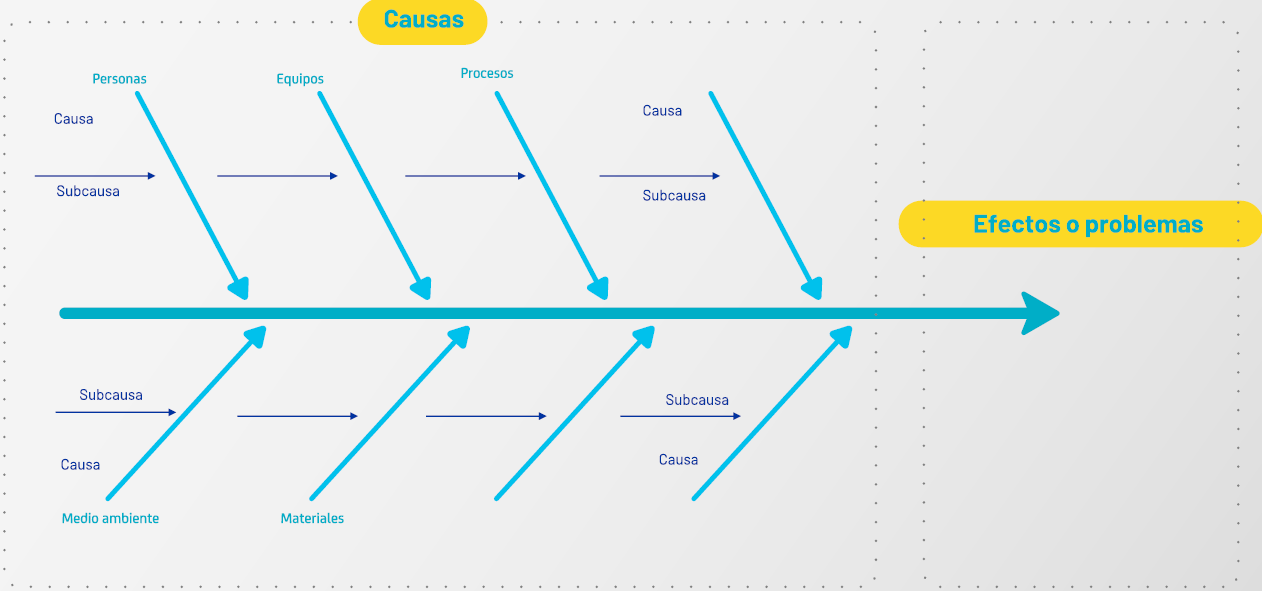
\includegraphics[width=1\textwidth]{espina.png}
			            \caption{Espina de pescado}
			            \label{fig:imagen2}
		            \end{figure}
	\item ¿Para qué sirve la
	metodología de análisis
	de causa-efecto en una
	organización?\newline
	El análisis de causa-efecto es una
	herramienta muy útil en las
	organizaciones debido a que permite
	identificar y analizar las posibles
	causas de un problema o una situación,
	a continuación se describen las
	utilidades de la metodología en una
	organización.
	      \begin{itemize}
			\newpage
		      \item Identificación de las causas de un problema\newline
		      El análisis de causa-efecto ayuda a las organizaciones a identificar las causas subyacentes de un problema en particular. Al hacer esto, se puede desarrollar una mejor comprensión del problema y se pueden tomar medidas para abordarlo adecuadamente.
				\item Mejora continua\newline
				Al utilizar el análisis de causa-efecto para identificar las causas de un problema, las organizaciones pueden desarrollar planes de mejora continua. Esto implica identificar y eliminar las causas raíz de los problemas para mejorar los procesos y las operaciones de la organización.
				\item Resolución de problemas\newline
				Al analizar las causas subyacentes de un problema, el análisis de causa-efecto ayuda a las organizaciones a desarrollar soluciones efectivas para resolver el problema. Estas soluciones se enfocan en abordar las causas raíz y no solo los síntomas del problema.
				\item Planificación y toma de decisiones\newline
				El análisis de causa-efecto se utiliza comúnmente en la planificación y toma de decisiones. Las organizaciones pueden utilizarlo para identificar los factores que afectan los resultados y, por lo tanto, tomar decisiones informadas para mejorar estos resultados.
			\end{itemize}
			\begin{figure}[H]
				\centering
				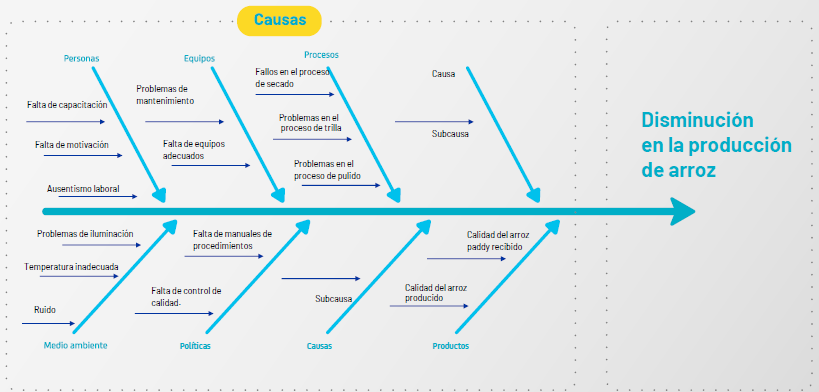
\includegraphics[width=1\textwidth]{espina2.png}
				\caption{Ejemplo de Espina de pescado}
				\label{fig:imagen2}
			\end{figure}
			\newpage

\section{Pareto}

El principio de Pareto es una herramienta de análisis y toma
de decisiones creada por Vilfredo Pareto (1848-1923)
a finales del siglo XIX en 1897. El economista y sociólogo
italiano, que estudió en la Universidad Politécnica de Turin en
ltalia, es considerado el padre fundador de lo que ahora se
llama "Principio de Pareto". Al estudiar la riqueza de su
país descubrió que sólo el 20\% de la gente poseía el 80\% de la
riqueza total. Luego aplicó esta ley a otros estados como
Rusia, Francia y Suiza y encontró los mismos resultados.
\begin{itemize}
	\item¿Comó surge el Principio de Pareto?
	      \begin{itemize}
		      \item El principio de Pareto surge de la observación de que el 20 \% de los clientes son responsables del 80\% de los efectos. Es decir en el mundo de los negocios, el 20 \% de los clientes son responsables del 80\% de la facturación. Al identificar este 20\% (los clientes más importantes) las empresas pueden prestarles más atención para ahorrar tiempo y dinero. Según Joseph Juran, el principio de Pareto se puede aplicar universalmente en el ámbito empresarial y se puede encontrar en todos los sectores de la sociedad. Incluso puedes utilizar el principio en la mayoría de las áreas de la vida diaria. Sin embargo, veremos que, tanto en el ámbito empresarial como en otros ámbitos, la relación 80/20 no siempre se respeta pero si da una idea de la realidad.
	      \end{itemize}
	\item El principio de Pareto como herramienta de control de calidad.\newline
	Una segunda aplicación, utilizada por Joseph Juran, es la del control
	y gestión de calidad en una línea de producción. Si el 20\% de
	Las fallas causan el 80\% de los problemas, la empresa puede concentrarse
	centrar sus esfuerzos en abordar las fallas en cuestión para
	para mejorar la calidad. También son válidas otras aplicaciones similares:
	\begin{itemize}
		\item El 20\% del tiempo de configuración de la máquina puede resolver el 80\% de los problemas;
		\item El 20\% de la línea de producción es responsable del 80\% del
		producto final.
	\end{itemize}
\newpage
	\item 	ESTUDIO DE CASO: UNA LÍNEA DE PRODUCCIÓN\newline
Introducción al problema\newline
Nuestro caso de estudio se refiere a una industria y su línea de
producción. En esta empresa, la línea de producción está
experimentando interrupciones recurrentes a lo largo del año. En conjunto
suman un total de 1033 horas, lo que supone poco más de un
mes de inactividad. Para compensar la pérdida de horas de trabajo,
el directivo, que advirtió que la dinámica no era lógica,
identifica las diez causas comunes de parada de línea. Luego estima
un tiempo de parada promedio (en horas) y proporciona un recuento
de ocurrencias para cada causa. Utilizando el principio de
Pareto, espera identificar los principales factores que perturban la línea
de producción.
\begin{table}[h!]
	\begin{tabular}{|l|l|l|l|l|}
	\hline 
	\multicolumn{1}{|p{155.83218pt}}{\raggedright Problemas (retraso en h)} & \multicolumn{1}{|p{61.730625pt}}{\raggedright Ocurrencias} & \multicolumn{1}{|p{48.18pt}}{\raggedright Total (h)} & \multicolumn{1}{|p{41.404686pt}}{\raggedright \%} & \multicolumn{1}{|p{60.225pt}|}{\raggedright Acumulado \ (\%)}\\ 
	\hline 
	\multicolumn{1}{|p{155.83218pt}}{\raggedright Configuraci\'on de la m\'aquina (7)} & \multicolumn{1}{|p{61.730625pt}}{\raggedright 56} & \multicolumn{1}{|p{48.18pt}}{\raggedright 392} & \multicolumn{1}{|p{41.404686pt}}{\raggedright 37,95} & \multicolumn{1}{|p{60.225pt}|}{\raggedright 37,95}\\ 
	\hline 
	\multicolumn{1}{|p{155.83218pt}}{\raggedright Recalibraci\'on (3)} & \multicolumn{1}{|p{61.730625pt}}{\raggedright 87} & \multicolumn{1}{|p{48.18pt}}{\raggedright 265} & \multicolumn{1}{|p{41.404686pt}}{\raggedright 25,27} & \multicolumn{1}{|p{60.225pt}|}{\raggedright 63,21}\\ 
	\hline 
	\multicolumn{1}{|p{155.83218pt}}{\raggedright Mala configuraci\'on (4)} & \multicolumn{1}{|p{61.730625pt}}{\raggedright 23} & \multicolumn{1}{|p{48.18pt}}{\raggedright 92} & \multicolumn{1}{|p{41.404686pt}}{\raggedright 8,91} & \multicolumn{1}{|p{60.225pt}|}{\raggedright 72,12}\\ 
	\hline 
	\multicolumn{1}{|p{155.83218pt}}{\raggedright Fuga de aceite de la m\'aquina (7)} & \multicolumn{1}{|p{61.730625pt}}{\raggedright 12} & \multicolumn{1}{|p{48.18pt}}{\raggedright 84} & \multicolumn{1}{|p{41.404686pt}}{\raggedright 8,13} & \multicolumn{1}{|p{60.225pt}|}{\raggedright 80,25}\\ 
	\hline 
	\multicolumn{1}{|p{155.83218pt}}{\raggedright Escasez de existencias (12)} & \multicolumn{1}{|p{61.730625pt}}{\raggedright 5} & \multicolumn{1}{|p{48.18pt}}{\raggedright 60} & \multicolumn{1}{|p{41.404686pt}}{\raggedright 5,81} & \multicolumn{1}{|p{60.225pt}|}{\raggedright 86,06}\\ 
	\hline 
	\multicolumn{1}{|p{155.83218pt}}{\raggedright Cambios de orden(4)} & \multicolumn{1}{|p{61.730625pt}}{\raggedright 15} & \multicolumn{1}{|p{48.18pt}}{\raggedright 60} & \multicolumn{1}{|p{41.404686pt}}{\raggedright 5,81} & \multicolumn{1}{|p{60.225pt}|}{\raggedright 91,87}\\ 
	\hline 
	\multicolumn{1}{|p{155.83218pt}}{\raggedright Fallo de compresor (7)} & \multicolumn{1}{|p{61.730625pt}}{\raggedright 4} & \multicolumn{1}{|p{48.18pt}}{\raggedright 28} & \multicolumn{1}{|p{41.404686pt}}{\raggedright 2,71} & \multicolumn{1}{|p{60.225pt}|}{\raggedright 94,58}\\ 
	\hline 
	\multicolumn{1}{|p{155.83218pt}}{\raggedright Huelga de empleados (24)} & \multicolumn{1}{|p{61.730625pt}}{\raggedright 1} & \multicolumn{1}{|p{48.18pt}}{\raggedright 24} & \multicolumn{1}{|p{41.404686pt}}{\raggedright 2,32} & \multicolumn{1}{|p{60.225pt}|}{\raggedright 96,90}\\ 
	\hline 
	\multicolumn{1}{|p{155.83218pt}}{\raggedright Corte de energ\'{\i}a (1)} & \multicolumn{1}{|p{61.730625pt}}{\raggedright 22} & \multicolumn{1}{|p{48.18pt}}{\raggedright 22} & \multicolumn{1}{|p{41.404686pt}}{\raggedright 2,13} & \multicolumn{1}{|p{60.225pt}|}{\raggedright 99,03}\\ 
	\hline 
	\multicolumn{1}{|p{155.83218pt}}{\raggedright Desglose general (2)} & \multicolumn{1}{|p{61.730625pt}}{\raggedright 5} & \multicolumn{1}{|p{48.18pt}}{\raggedright 10} & \multicolumn{1}{|p{41.404686pt}}{\raggedright 0,97} & \multicolumn{1}{|p{60.225pt}|}{\raggedright 100,00}\\ 
	\hline 
	\multicolumn{1}{|p{155.83218pt}}{\raggedright TOTAL} & \multicolumn{1}{|p{61.730625pt}}{\raggedright 230} & \multicolumn{1}{|p{48.18pt}}{\raggedright 1033} & \multicolumn{1}{|p{41.404686pt}}{\raggedright 100,00} & \multicolumn{1}{|p{60.225pt}|}{}\\ 
	\hline 
	
	\end{tabular}
	\end{table}	
	      \begin{figure}[H]
		      \centering
		      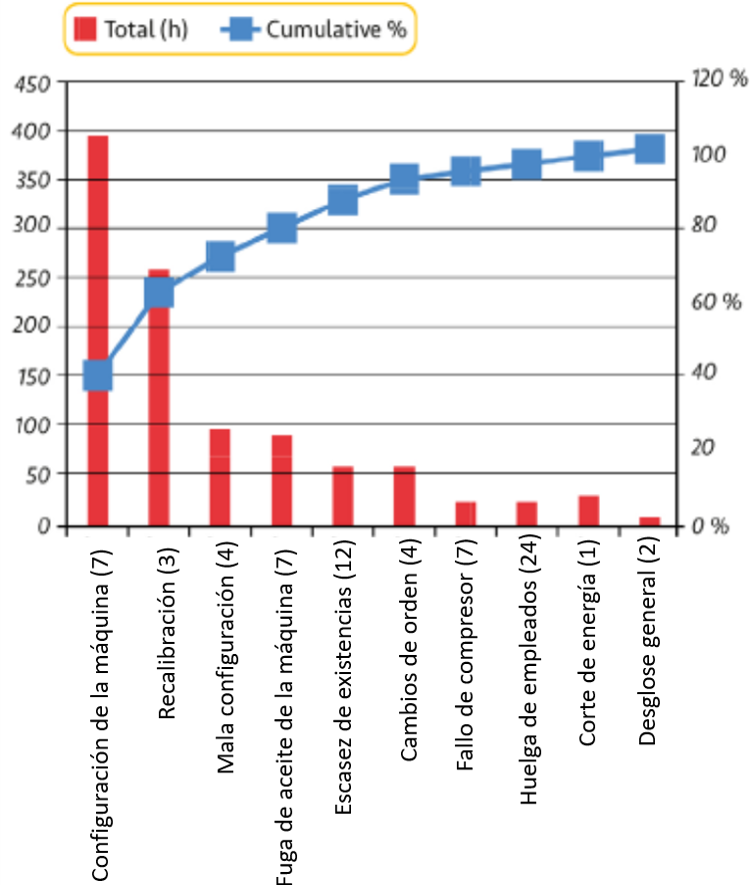
\includegraphics[width=0.7\textwidth]{Grapich.png}
		      \caption{Gráfico de la línea de producción de la industria}
		      \label{fig:imagen2}
	      \end{figure}

	\item Identificar los factores importantes\newline
	El principio de Pareto funciona particularmente bien en este caso
	porque una minoría de factores causa la mayoría de los problemas.
	En concreto, casi el 30\% de los factores provocan el 72\% de los retrasos
	en la línea de producción. Observe que hay otras dos proporciones
	cercanas a 80/20:
	      \begin{enumerate}
		      \item Al considerar las dos mayores causas (20\%), el
			  porcentaje de retrasos es del 63\%;
		      \item Si se consideran los cuatro mayores problemas (40\%), el
			  porcentaje de retrasos es del 80\%.
	      \end{enumerate}\newpage
		  \item ¿Cuál es la mejor proporción? \newline
		   Está claro que la proporción general del 30\% de los factores que
	causan el 72\% de los retrasos es la más cercana al principio de Pareto.
	Desafortunadamente, esto no resuelve todos los problemas:
	\begin{enumerate}
		\item En primer lugar, nos quedan muchos factores problemáticos
		que ajustar, pero elegir centrarnos en la primera proporción (dos
		cuestiones principales) nos centraríamos en una minoría de causas
		que causan el máximo número de consecuencias, que es precisamente
		el objetivo del principio de Pareto;
		\item En segundo lugar, si el director de la planta quiere solucionar tantos
		problemas como sea posible, tiene todos los motivos para centrarse en el
		tercer ratio, corrigiendo el 40\% de las causas que provocan el 80\% de
		los retrasos en la línea de producción.
	\end{enumerate}
		  \section{De flujo}

		  \section{Dispersión}
		  \section{Análisis de tendencia}



\newpage
\end{itemize}
\bibliographystyle{apacite}
\nocite{*}
\bibliography{instrumentos}

\end{document}